\chapter{Tecnologie Implicate}

Lo sviluppo del progetto \`e stato svolto nell'ambiente Raspbian\cite{Raspbian}
una distribuzione Debian\cite{Debian} che gira sul dispositivo RasperryPi\cite{Raspberry}.
Inoltre sono state adottate diverse tecnologie, recenti
e non, nel campo della creazione di applicazioni(Electron \cite{Electron-website},
OpenCV \cite{OpenCV-website}, GoogleSpeechRecognition \cite{GoogleSTT-website}),
dei web server (NodeJS \cite{NodeJS-website}, Express \cite{Express-website}, Mustache \cite{Mustache}),
della gestione dati (MySQL \cite{MySQL}).
Inoltre sono stati adottati diversi linguaggi di programmazione (JavaScript \cite{JavaScript}, Python \cite{Python})
e piattaforme per la gestione distribuita di progetti softwave (GitLab \cite{git-website}).

\section{Hardware}
\subsection{RasperryPi}
RaspberryPi \`e un calcolatore elettronico, montato su una singola scheda elettornica,
caratterizzato dal basso costo, dal consumo energetico ridotto e, per le sue
dimensioni ridotte, dalla facile portabilit\`a.
Rilasciato per la prima volta nel 2012 \`e diventato un prodotto utilizzato per una moltitudine
di progetti sia aziendali che casalinghi.
Il modello usato durante lo stage \`e RaspberryPi 3 model B e monta:
\begin{itemize}
\item 1 porta HDMI
\item 1 porta LAN
\item 1 uscita Aux
\item 4 porte USB
\item 40 pin General Purpose Input/Output(GPIO)
\item 1 scheda di rete wirless
\item Alimentazione microUSB 5V
\item un bus camera serial interface(CSI), ovvero una porta per telecamere con Flexible flat cable(FFC)
\item ingresso per microSD
\end{itemize}
Il sistema operativo per Raspberry deve essere installato su una miscroSD opportunamente formattata
e configurata con un Master Boot Record (MBR).

\subsection{Periferiche}
Nella creazione delle applicazioni per il Magic Mirror sono stati usati diverse periferiche, tra cui un microfono
USB, per catturare la voce in input e un componente Skydriver Touch Board (94mm x 122mm) di Piromoni collegabile tramite
i 40 pin GPIO del calcolatore principale, per catturare input fisici tramite il movimento delle dita sulla scheda.

\section{Software}
\subsection{Raspbian}
Raspbian \`e una distribuzione del sistema operativo Debian, completamente libero,
ottimizzato per Raspberry.
Fu sviluppato da Mike Thompson e Peter Green come progetto non affiliato alla compagnia RaspberryPi
fundation, pensato apposta per la bassa potenza dei processori Advanced RISC Machine(ARM) montati sul
dispostivo.
La prima versione venne rilasciata nel 2012.

\subsection{Electron}
Electron \`e un Framework open source rilasciato per la prima volta nel 2013, ma la prima versione
stabile \`e uscita solo di recente. \`E disponibile sui sistemi operativi Window, MacOS e Linux ed \`e scritto
in C++ e Javascript. Il framework permette la creazione di interfacce grafiche (GUI) per
applicazioni multi-piattaforma, utilizzando teconologie gi\`a esistenti per lo sviluppo
del lato client e del lato server (Javascript, NodeJS, V8 \cite{V8}).
All'avvio di Electron viene inizializza una pagina con Chromium \cite{Chromium}(il quale viene installato con l'applicazione)
nel quale viene mostrata una pagina web, e un server in NodeJS che si occupa di trasmettere e interagire con il primo.
Un'applicazione Electorn ha bisongo di 3 componenti principali:
\begin{itemize}
\item Il package.json, un file JSON, che deve contenere almeno il nome dell'applicazione,
la versione dell'applicazione creata, la descrizione di quest'ultima e il
 nome del file principale dell'applicazione (necessaria per l'avvio)
\begin{lstlisting}
{
  "name": "magicmirror",
  "version": "2.1.1",
  "description": "The open source smart platform",
  "main": "js/electron.js"
}
\end{lstlisting}
\item Un file HTML che contiene il template della pagina mostrata dall'applicazione
\item Un file JavaScript che contiene il codice di esecuzione dell'applicazione come ad esempio la
creazione di una finestra o la visualizzazione di una pagina.
\end{itemize}

\subsection{OpenCV}
OpenCV (Open Source Computer Vision Library) \`e una libreria software sviluppata intorno al 2000
utilizzata nell'ambito della visione in tempo reale
da parte di una macchia per mezzo di input digitali, ottenuti tramite telecamera o fotocamera.\\
La libreria \`e disponibile per i linguaggi C++(linguaggio in cui \`e scritta e dunque di cui ha l'interfaccia primaria), C, Python e Java e
per diversi sistemi operativi, compresi quelli specifici per i dispositivi mobili.\\
OpenCV prende in input un'immagine o uno stream (come un video o una serie di immagini) e, utilizzando algoritmi
 implementati al suo interno, riconosce oggetti o specifiche forme.
Inoltre si pu\`o aumentarne la capacit\`a
applicando algoritmi di Machine Learning per individuare e riconoscere oggetti specifici.

\subsection{Google Speech API}
Negli ultimi anni Google ha ampliato sempre di pi\`u il suo catalogo per quanto rigarda
i servizi cloud e web API.
Tra questi si pu\`o individuare anche Google Speech API, il quale \`e un
servizio che, ricevendo in input un file o uno stream audio, ottenuto per mezzo di un
dispositivo di audio input, traduce il parlato in testo scritto tramite algoritmi avanzati
di riconoscimento della voce.\\
L'API supporta oltre 110 lingue e si possono usare su diverse piattaforme dato che
le librerie sono disponibili nei linguaggi C\#, GO, Java, Node.JS, PhP, Python e Ruby.
Inoltre Google Speech To Text dispone di alcune varianti:
\begin{itemize}
\item Una con interfaccia REpresentational State Transfer(REST), che comunica per mezzo di URI
\item Una con gRPC, un sistema di chiamata di procedura remota
\end{itemize}

\iffalse
\section{Model-View-Design}
Il Model-View-Design (MVC) \`e un pattern architetturale che suddivide lo sviluppo di un'applicazione web in 3 parti:
\begin{itemize}
\item Model(Modello), sono oggetti che rappresentano lo stato dell'applicazione e operazioni logiche da eseguire sul primo. Di solito
lo stato del modello viene estratto, manipolato per mezzo di operazioni e salvato da un database con cui comunicano,
oppure passato al controller.
\item Controller, \`e un'interfaccia che comunica tra il Model, la View e l'Utente. Il suo compito \`e di gestire le richieste dell'utente,
il quale comunica tramite input ed interazioni, utilizzando il modello che rientra nel dominio
dei dati inerente alla richiesta e selezionando una View per il rendering dell'interfaccia utente.
\item View(Visualizzazione), ha il compito di far visualizzare all'utente i dati estratti tramite un'interfaccia grafica, che viene creata
partendo da un modello HTML.\\[2\baselineskip]
\end{itemize}
\begin{figure}[H]
    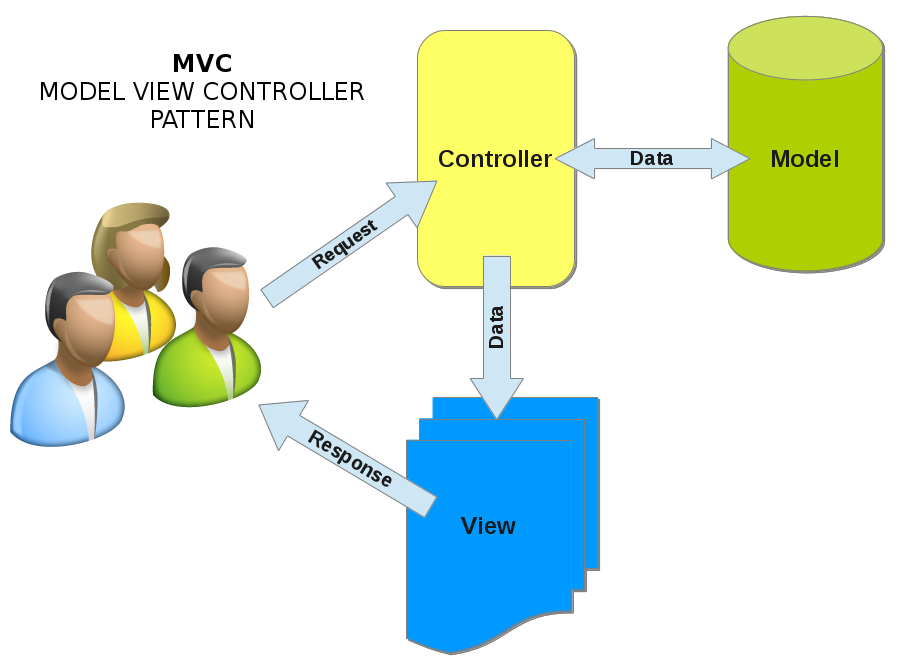
\includegraphics[width=0.9\textwidth]{mvc}
    \caption{MVC Pattern}
\end{figure}
\fi

\subsection{NodeJS}
NodeJS \`e una piattaforma open source, utilizzata per progettare il backend di un server web, ovvero
la parte del sistema che contiene applicazioni e programmi con cui l'utente non interagisce e
che ne permette l'effettivo funzionamento e, nel caso, la manipolazione e l'elaborazione
dei dati, sfruttando il motore JavaScript V8 sviluppato da Google.\\
NodeJS esegue delle operazioni al verificarsi di uno specifico evento, che pu\`o essere un accesso ad una porta
del server o la richiesta di una pagina.
Per gestire i pacchetti di questo framework viene utilizzato NPM\cite{NPM}, uno strumento che permette
di scaricare ed installare librerie private o pubbliche salvate su un database.
\\[1\baselineskip]

\subsubsection{Express}
Express \`e un framework per NodeJS che permette di creare applicazioni Web e API in JavaScript.
Il software viene usato per creare e gestire il backend di un server, che \`e composto di 3 entit\`a importanti:
\begin{itemize}
\item il Routing, utilizzato per determinare come il server debba rispondere ad un determinato metodo di richiesta,
ricevuta sottoforma di URI, inoltrando la richiesta alla funzione del controller del modello a cui fa rifermento.
\item i Modelli, creati per ogni entit\`a-oggetto che esiste all'interno del server, ad ognuno dei quali viene associato
un controller. Inoltre, tramite i modelli si accede al databse per estrarre i dati e spedirli al controller per
la manipolazione, ricevendoli successivamente modificati e salvandoli, se necessario.
\item il Controller, che definisce le funzioni associate ad un determinato modello.
\\[2\baselineskip]
\end{itemize}

\subsection{JavaScript}
Javascript \`e un linguaggio di programmazione di alto livello per oggetti ed eventi, che \`e supportato da tutti i browser
per lo scripting delle pagine web, conosciuto per l'utilizzo in programmazione procedurale e per la programamzione orientata ad oggetti.
Inzialmente usato per il lato client ha subito un'evoluzione che lo ha portato ad essere utilizzato per lo sviluppo di backend e web app.
Gli oggetti in Javascript vengono creati a livello di codice collegando metodi e propriet\`a ad altri oggetti, anche vuoti, a tempo
di esecuzione.

\\[2\baselineskip]
ECMAJavascript(ES) \`e lo standard di Javascript che negli ultimi anni ha sviluppato ed evoluto il linguaggio in diverse verisoni.
In tutte il problema pi\`u trattato \`e il fatto che Javascript \`e asincrono, ovvero non attende il completamento di alcune
operazioni prima di eseguire le funzioni successive. QUesto avviene perch\`e le chiamate di funzioni non vengono fatte direttamente, ma vengono
fatte via messaggi, i quali vengono salvati in una coda di messaggi e vengono spediti sequenzialmente ad uno stack di chiamata dove
viene salvata la corrispondente funzione per l'esecuzione. Questo metodo rende il linguaggio asincorno perch\`e le funzioni e gli eventi
vengono eseguiti in successione senza attendere il termine dalla precedente.
\\[1\baselineskip]Le soluzioni adottate in ECMA Javascrit 5 (ES5), sono l'utilizzo delle callback,
funzioni passate come parametro alla funzione principale che a loro volta avevano come paramentro il risultato, in modo da poter eseguire le operazioni
solo dopo che la funzione chiamante avesse prodotto l'output. Il problema di questo approccio \`e stato il fenomeno "Callback Hell", ovvero Callback che chiamano a loro volta
altre Callback creando funzioni annidate pi\`u volte.
\\[1\baselineskip]
In ECMA Javascript 6 (ES6) sono state introdotte le Promises, ovvero al posto di far tornare una funzione Callback, ritorna una Promise(Promessa),
la quale garantisce che una variabile/oggetto avr\`a un ritorno, mettendo cosi la funzione in attesa fino al ricevimento del valore o di un errore.
Sono tutt'ora in via di sviluppo nuove versioni di Javascript.
\\[2\baselineskip]
\begin{figure}[h]
    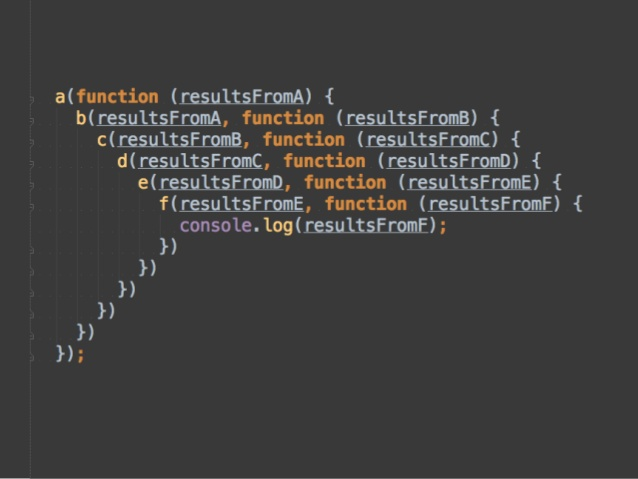
\includegraphics[width=1\textwidth, height=0.4\textheight]{callbackhell}
    \caption{Esempio di Callback Hell}
\end{figure}

\subsection{Python}
Python \`e un linguaggio di programmazione open source, ad alto livello con semantica dinamica, orientato ad oggetti, usato
per sviluppo di applicazioni, scripting e per collegare componenti tra di loro.\\[1\baselineskip]
Come molti altri linguaggi supporta moduli e pacchetti anche sviluppati da terzi, salvati in una repository pubblica,
attraverso un suo gestore di pacchetti Pip Installs Packages o Pip Installs Python (pip, acronimo ricorsivo).
\\[1\baselineskip]
Inoltre con Python \`e possibile creare ambienti isolati per l'utilizzo di pacchetti e moduli senza doverli installare all'interno del sistema.
Per poterlo fare \`e disponibile virtualenv, uno strumento Python che permette, appunto, di creare ambienti virtuali (virtual enviroments).
Questo linguaggio \`e stato particolarmente utile per l'interfacciamento con la telecamera e la Touch Board avendo una librerie
apposite per gestirle.
\\[2\baselineskip]

\subsection{GitLab}
GitLab \`e un web repository che implementa le funzionalit\`a offerte dal software Git e altri
servizi tra i quali la possibilit\`a di creare wiki e un servizio di issue tracking, utile per tenere traccia
di evenutali richieste o problemi.
Il software Git \`e stato creato da da Linus Torvalds nel 2005 per la gestione e il versionamento del codice in Linux.
Git \`e, in sostanza, un grafo diretto aciclico di oggetti, ognuno con un'identificativo univoco, ed \`e composto da 4 parti principali:
\begin{itemize}
\item i Blob, insieme di bytes che contengono i dati all'inteno dei file.
\item i Trees, sono le cartelle che contengono, all'interno, un lista di file con alcuni bit i quali fanno riferimento al
rispettivo blob o ad un'altro Tree.
\item i Tag, sono etichette con dati aggiuntivi per identificare e gestire i nodi.
\item i Commit, collegano pi\`u oggetti Tree ad uno storico nel quale sono salvati anche i nomi di tutti i commits parenti.
\end{itemize}
